% ---
% Capa
% ---
\imprimircapa
% ---

% ---
% Folha de rosto
% (o * indica que haverá a ficha bibliográfica)
% ---
\imprimirfolhaderosto*
% ---

% ---
% Inserir a ficha bibliografica
% ---
% http://ficha.bu.ufsc.br/
\begin{fichacatalografica}
	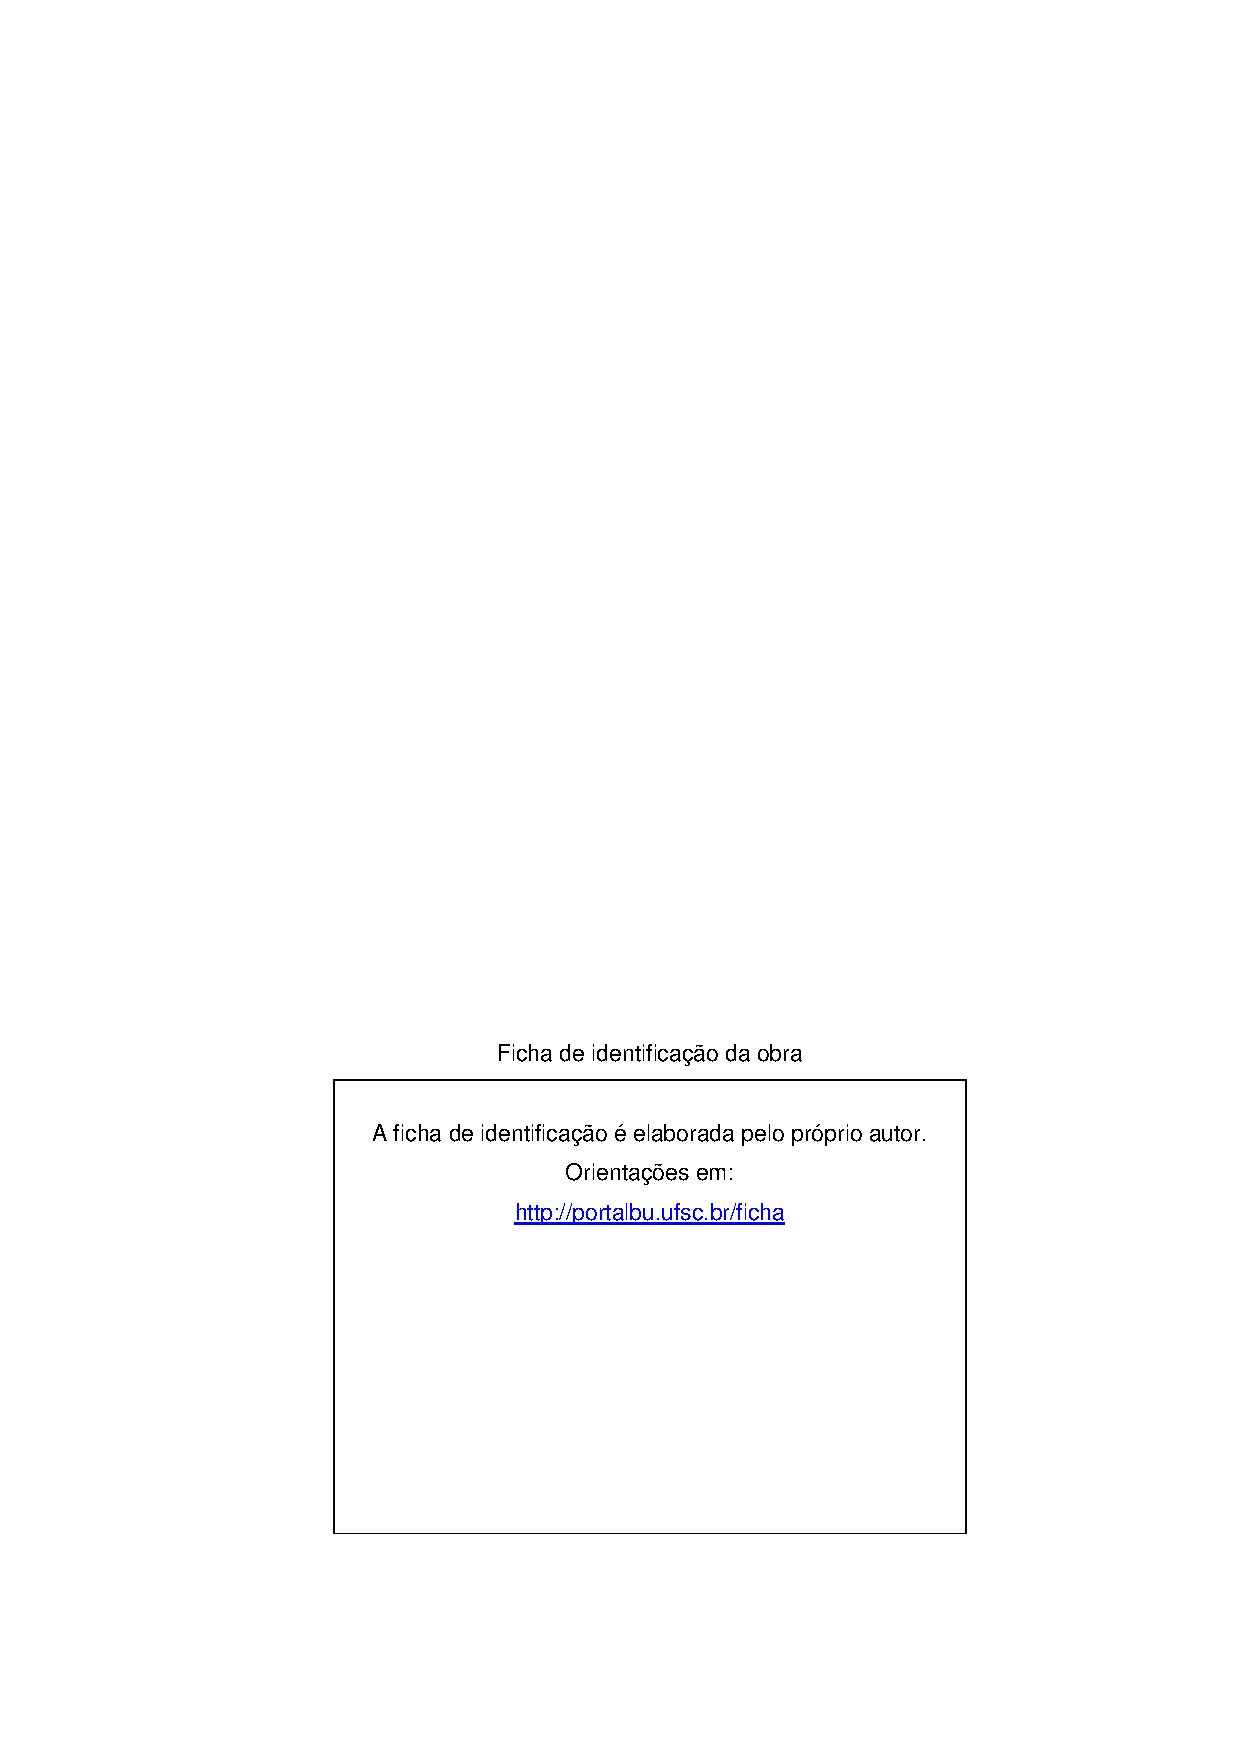
\includepdf{beforetext/Ficha_Catalografica.pdf}
\end{fichacatalografica}
% ---

% ---
% Inserir folha de aprovação
% ---
\begin{folhadeaprovacao}
	\OnehalfSpacing
	\centering
	\imprimirautor\\%
	\vspace*{10pt}		
	\textbf{\imprimirtitulo}%
	\ifnotempty{\imprimirsubtitulo}{:~\imprimirsubtitulo}\\%
	%		\vspace*{31.5pt}%3\baselineskip
	\vspace*{\baselineskip}
	%\begin{minipage}{\textwidth}
	O presente trabalho em nível de \imprimirnivel~foi avaliado e aprovado por banca examinadora composta pelos seguintes membros:\\
	%\end{minipage}%
	\vspace*{\baselineskip}
	Prof. Dr. Odorico Machado Mendizabal \\
	Universidade Federal de Santa Catarina \\
	\vspace*{\baselineskip}
	Prof.(a) xxxx, Dr(a).\\
	Instituição xxxx\\
        \vspace*{\baselineskip}
	Prof.ª Dr.ª Atslands Rego da Rocha \\
	Universidade Federal do Ceará \\
	\vspace*{2\baselineskip}
	\begin{minipage}{\textwidth}
		Certificamos que esta é a \textbf{versão original e final} do trabalho de conclusão que foi julgado adequado para obtenção do título de \imprimirformacao.\\
	\end{minipage}
	%    \vspace{-0.7cm}
	\vspace*{\fill}
	\assinatura{\OnehalfSpacing Coordenação do Programa de Pós-Graduação}
	\vspace*{\fill}
	\assinatura{\OnehalfSpacing\imprimirorientador \\ \imprimirorientadorRotulo}
	%	\ifnotempty{\imprimircoorientador}{
	%	\assinatura{\imprimircoorientador \\ \imprimircoorientadorRotulo \\
	%		\imprimirinstituicao~--~\imprimirinstituicaosigla}
	%	}
	% \newpage
	\vspace*{\fill}
	\imprimirlocal, \imprimirano.
\end{folhadeaprovacao}
% ---

% ---
% Dedicatória
% ---
\begin{dedicatoria}
	\vspace*{\fill}
	\noindent
	\begin{adjustwidth*}{}{5.5cm} 
		\raggedleft       
		Dedico este trabalho a todos os meus professores, 
sendo, meus pais, os maiores entre eles.
	\end{adjustwidth*}
\end{dedicatoria}
% ---

% ---
% Agradecimentos
% ---
\begin{agradecimentos}
    Neste momento, sinto uma gratidão imensa por cada pessoa que fez parte desta jornada. Agradeço de coração aos meus pais e à minha namorada, cujos amores incondicionais e apoios constantes foram a base sólida sobre a qual construí meus sonhos e conquistas. Sem vocês, nada disso teria sido possível.

    À UFSC (Universidade Federal de Santa Catarina) e a todos os seus membros, expresso meu profundo agradecimento. Cada professor, funcionário e colega desempenhou um papel crucial no meu crescimento acadêmico. Através do ensino de qualidade, das valiosas ferramentas e dos recursos disponibilizados, pude adquirir o conhecimento necessário para realizar este trabalho.

    Em especial, minha orientadora Patrícia Della Méa Plentz, você foi uma inspiração e guia ao longo dessa jornada. Sua dedicação, sabedoria e orientação foram fundamentais para a construção desta qualificação. Agradeço por compartilhar seu conhecimento, suas perspectivas e por me motivar a alcançar meu melhor desempenho. Sua generosidade em investir tempo e energia em minha formação é um presente inestimável.

    Um agradecimento especial à LexisNexis, em especial a Mauro Marques e Alysson Oliveira. Sua colaboração e apoio foram cruciais para o desenvolvimento deste trabalho. Suas expertise e capacidade analítica, com seu suporte técnico e encorajamento constante, enriqueceram imensamente minha pesquisa. Sou profundamente grato(a) a ambos por sua dedicação e por acreditarem no potencial deste projeto.


    A todos vocês, meus pais, minha namorada, minha orientadora e a equipe da LexisNexis, sou profundamente grato(a). Seus ensinamentos, apoio e encorajamento foram a força motriz que me impulsionou a superar desafios e alcançar meus objetivos. Cada palavra de incentivo, cada gesto de apoio e cada momento de aprendizado deixaram uma marca indelével em minha vida acadêmica e pessoal.

    Expresso minha sincera admiração e gratidão por cada contribuição que fizeram em minha jornada. Vocês são verdadeiros pilares em minha vida, e sou grato(a) por terem acreditado em mim e por terem compartilhado esse caminho comigo.

\end{agradecimentos}
% ---

% ---
% Epígrafe
% ---
\begin{epigrafe}
	\vspace*{\fill}
	\begin{flushright}
		\textit{''A educação é a arma mais poderosa que \\
            você pode usar para mudar o mundo.'' \\
            (Nelson Mandela)
            }
	\end{flushright}
\end{epigrafe}
% ---

% ---
% RESUMOS
% ---

% resumo em português
\setlength{\absparsep}{18pt} % ajusta o espaçamento dos parágrafos do resumo
\begin{resumo}
	\SingleSpacing
	Este trabalho apresentou o desenvolvimento e a avaliação de uma arquitetura modular para ambientes de computação em névoa, projetada para suportar comunicação direta entre diferentes domínios e integrar dispositivos de borda, nós de névoa e a nuvem, tomando como referência o modelo do OpenFog Consortium. A solução foi construída com base nos pilares de escalabilidade, abertura, autonomia, programabilidade e hierarquia, considerando o contexto de cidades inteligentes. A proposta incorporou abstração de protocolos para permitir interoperabilidade entre diferentes tecnologias de comunicação, além de um mecanismo de balanceamento dinâmico de carga e agregação de dados para otimizar o uso de recursos e reduzir o tráfego de dados para a nuvem. A metodologia envolveu a simulação de dois dias de operação contínua, com dispositivos distribuídos em dois domínios de névoa e geração periódica de dados, analisando métricas de latência, consumo de memória, throughput, taxa de entrega e fator de agregação. Os resultados indicaram latência ponta a ponta média de 15,6 ms, taxa de entrega de 100\% e redução de aproximadamente 99,97\% nas requisições à nuvem, mantendo desempenho compatível com aplicações sensíveis ao tempo. A comparação com trabalhos como o EXEGESIS evidenciou diferenças no gerenciamento de serviços e na flexibilidade de adaptação a novos cenários, destacando vantagens na separação entre a camada de aplicação e a de protocolos. Entre as perspectivas futuras estão a implementação de autenticação e criptografia ponta a ponta, estratégias de recuperação automática e validação da arquitetura em domínios como saúde conectada e transporte inteligente.
	
	\textbf{Palavras-chave}: computação em névoa. interoperabilidade. balanceamento de carga.
\end{resumo}

% resumo em inglês
\begin{resumo}[Abstract]
	\SingleSpacing
	\begin{otherlanguage*}{english}
		This research presented the development and evaluation of a modular architecture for fog computing environments, designed to support direct communication between different domains and to integrate edge devices, fog nodes, and the cloud, taking the OpenFog Consortium reference model as a guideline. The solution was built on the pillars of scalability, openness, autonomy, programmability, and hierarchy, within the context of smart cities. The proposal incorporated protocol abstraction to enable interoperability among different communication technologies, along with a dynamic load balancing mechanism and data aggregation to optimize resource usage and reduce cloud traffic. The methodology involved simulating two days of continuous operation, with devices distributed across two fog domains and generating periodic data, analyzing metrics such as latency, memory consumption, throughput, delivery rate, and aggregation factor. The results indicated an average end-to-end latency of 15.6 ms, a delivery rate of 100\%, and approximately 99.97\% reduction in cloud requests, maintaining performance compatible with time-sensitive applications. Comparison with works such as EXEGESIS highlighted differences in service management and adaptability to new scenarios, with advantages in the separation between the application and protocol layers. Future perspectives include implementing end-to-end authentication and encryption, automatic recovery strategies, and validating the architecture in domains such as connected healthcare and intelligent transportation.

		\textbf{Keywords}: fog computing. interoperability. load balancing.
	\end{otherlanguage*}
\end{resumo}


%% resumo em francês 
%\begin{resumo}[Résumé]
% \begin{otherlanguage*}{french}
%    Il s'agit d'un résumé en français.
% 
%   \textbf{Mots-clés}: latex. abntex. publication de textes.
% \end{otherlanguage*}
%\end{resumo}
%
%% resumo em espanhol
%\begin{resumo}[Resumen]
% \begin{otherlanguage*}{spanish}
%   Este es el resumen en español.
%  
%   \textbf{Palabras clave}: latex. abntex. publicación de textos.
% \end{otherlanguage*}
%\end{resumo}
%% ---

{%hidelinks
	\hypersetup{hidelinks}
	% ---
	% inserir lista de ilustrações
	% ---
	\pdfbookmark[0]{\listfigurename}{lof}
	\listoffigures*
	\cleardoublepage
	% ---
	
	% ---
	% inserir lista de quadros
	% ---
	\pdfbookmark[0]{\listofquadrosname}{loq}
	\listofquadros*
	\cleardoublepage
	% ---
	
	% ---
	% inserir lista de tabelas
	% ---
	\pdfbookmark[0]{\listtablename}{lot}
	\listoftables*
	\cleardoublepage
	% ---
	
	% ---
	% inserir lista de abreviaturas e siglas (devem ser declarados no preambulo)
	% ---
	\imprimirlistadesiglas
	% ---
	
	% ---
	% inserir lista de símbolos (devem ser declarados no preambulo)
	% ---
	\imprimirlistadesimbolos
	% ---
	
	% ---
	% inserir o sumario
	% ---
	\pdfbookmark[0]{\contentsname}{toc}
	\tableofcontents*
	\cleardoublepage
	
}%hidelinks
% ---